\documentclass{article}

%packages
\usepackage[LGR]{fontenc}
\usepackage[english,greek]{babel}
\usepackage{amsfonts}
\usepackage{mathtools}
\usepackage{pifont}
\usepackage{amsmath}
\usepackage{listings}

%commands
\newcommand{\blank}[1]{\hspace*{#1}}
\newcommand{\mysp}{\blank{0.3cm}}
\newcommand{\lt}[1]{\latintext #1\greektext}
\newcommand{\gt}[1]{\greektext #1\latintext}
\newcommand{\blt}[1]{\lt{\textbf{#1}}}
\newcommand{\tb}[1]{\textbf{#1}}
\newcommand{\ti}[1]{\textit{#1}}

%default parameters
\setcounter{MaxMatrixCols}{20}
\setlength{\parindent}{0pt}

%header
\title{\huge \tb{
    Εργασία Ευφυή Αυτόνομα Συστήματα\\
    \hfill\\
    Καθοδήγηση ρομπότ σε άγνωστο περιβάλλον
}}
\author{
    \LARGE Αποστολούδης Αντώνης \blank{1cm} Κύδρος Ασημάκης\\
    \LARGE 3897 \blank{5cm} 3881\\
    \LARGE \lt{antoapos@csd.auth.gr \blank{1cm} asimakis@csd.auth.gr}
}
\date{\LARGE \today}

\begin{document}
\maketitle
\Large

\section*{Κατασκευή του Ρομπότ}

Ορίζουμε το ρομπότ ώστε να διαθέτει:
\begin{itemize}
    \item 3 αισθητήρες φωτός, 2 μπροστινούς ισαπέχοντες στα αριστερά και δεξιά του και έναν πάνω από το κέντρο βάρος του
    \item 12 \lt{SONAR}, ισαπέχοντα σε μια ζώνη γύρω από το σώμα του.
\end{itemize}

\newpage 

\section*{Συμπεριφορές}

\begin{itemize}
    \item \blt{halt}:\\
    Το ρομπότ, σε κάθε χτύπο του ρολογιού (\lt{tempo}) κοιτάει αν η τιμή του κεντρικού αισθητήρα φωτός έχει ξεπεράσει μια συγκεκριμένη τιμή (\lt{globalMax}).
    Αυτή η τιμή βρέθηκε πειραματικά, ώστε το ρομπότ να σταματάει σε απόσταση με τη προβολή της λάμπας περίπου 0.2\lt{m}. 
    \item \blt{march}:\\
    Κατά την ελεύθερή του κίνηση, το ρομπότ προσπαθεί ταυτοχρόνως να βελτιώσει την απόκλιση της απόστασής του με τη λάμπα αλλά και της γωνίας του με τη λάμπα. Το πρώτο γίνεται ορίζοντας \[V_{translational} \propto \frac{1}{1 + c}\] όπου $c$ η μέτρηση του κεντρικού αισθητήρα φωτός στο δεδομένο \lt{tempo}. Καθώς το κλάσμα μικραίνει όσο το $c$ μεγαλώνει, η ταχύτητά του όσο πλησιάζει το φώς ολοένα και μικραίνει.
    Αναλόγως, ορίζουμε \[V_{rotational} \propto l - r\] όπου $l, r$ οι μετρήσεις του αριστερού και δεξιού αισθητήρα φωτός αντιστοίχως στο δεδομένο \lt{tempo}. Εδώ, εκτός από το ότι η ταχύτητα περιστροφής μικραίνει όσο οι δυο τιμές τείνουν στην ισοτιμία (άρα το ρομπότ κοιτά ευθεία προς τη λάμπα), αλλά και το πρόσημο της διαφοράς δείχνει αν η περιστροφή πρέπει να γίνει δεξιόστροφα ή αριστερόστροφα:
    \begin{figure}[h]
        \centering
        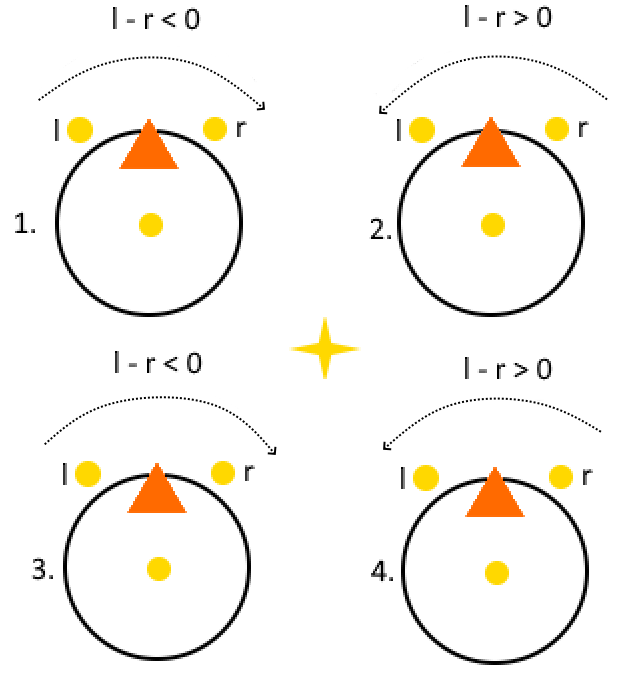
\includegraphics[scale=0.5]{images/align.png}
        \caption{Σε κάθε περίπτωση, το ρομπότ περιστρέφεται προς το φώς.}
        \label{fig:enter-label}
    \end{figure}

    \newpage 
    
    \item \blt{orbit}: O αλγόριθμος της περιφοράς γύρω από εμπόδιο δεν παρεκκλείνει ουσιαστικά από αυτόν της θεωρίας. Το ρομπότ, για να μπει σε περιφορά, ''κοιτάει'' συνεχώς στο μπροστινό του τεταρτοκύκλιο μέσω των \lt{SONAR} μέχρι να εντοπίσει εμπόδιο.
    \begin{figure}[h]
        \centering
        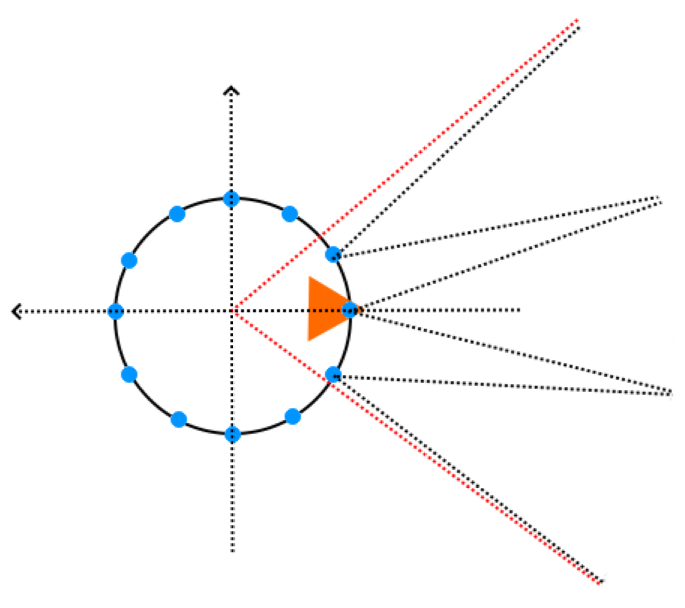
\includegraphics[scale=0.5]{images/vision.png}
        \caption{Η περιοχή ανίχνευσης εμποδίων.}
        \label{fig:enter-label}
    \end{figure}
    Με το που καταγράψει εμπόδιο σε επικίνδυνα κοντινή απόσταση (κάνει ''\lt{bump}''), καταγράφει την τωρινή του $c$ και εκτελεί περιφορά μέχρι να την ξεπεράσει. 
\end{itemize}
    
\newpage

\section*{Αλγόριθμος \lt{iBug}}

Η ιεραρχία των κινήσεων του ρομπότ, από μεγαλύτερη προς μικρότερη προτεραιότητα, είναι \lt{halt, orbit, march}. Έτσι, ο ψευδοκώδικας της λειτουργίας του ρομπότ είναι:
{
    \latintext
    \large
    \begin{lstlisting}
    repeat every tempo:
        if c over the global max then 
            halt
        else if c below the local max then 
            orbit the nearest object
        else if the robot bumped then 
            set local max to c
        else
            march towards the light
    end repeat    
    \end{lstlisting}
}

Παρέχουμε 3 περιβάλλοντα, 2 με κυρτά εμπόδια και 1 με κοίλο. Μέσω αυτού του αλγορίθμου, τα αποφεύγει όλα επιτυχώς και ολοκληρώνει τον στόχο του.
    
    
    
\end{document}
